\subsection{RQ3: What is the range of possible effects of bad ESP ?}\label{sect:rq3}
 This analytical study  of this section  examines the coefficients of the terms in the COCOMO equation
 to see what effect changes in KSLOC have on COCOMO's effort prediction.
 This study is motivated as follows:
 \bi
 \item
 Recall
from the introduction that this exponential nature of the COCOMO equation 
made it seem as if COCOMO would be most suceptible to errors in lines of code.
\item
Yet we saw in the last section that COCOMO is remarkably {\em insensitive} to LOC errors.
\ei
One explanation for the strange results of the last section is that the coeffecients
on the exponential term in   COCOMO   are so small that COCOMO does not
react poorly to LOC errors.
The analytical study of this section shows that this is indeed the case. In turns
out that for most projects, the COCOMO effort estimate is effectively linear, and not exponential
on SLOC.
The proof of this is somewhat somewhat technical but the main result is \eq{sf3} 
that shows the range  of the exponential coefficients for  COCOMO projects. Note that rarely are those coefficients very very large-- so much so that when we graph the changes in effort due to increased SLOC, the scale-up
is much less than exponential (see \fig{lowerupper}).



The coeffecients learned by Boehm in 2000 for the
COCOMO were based on an analysis of 
161 projects from commercial, aerospace, government, and non-profit organizations~\cite{boehm00b}. At the time of that analysis,
those  projects   were of size 20 to 2000 KSLOC (thousands of lines of code) and took between 100 to 10000 person months to build.
Recall from \eq{one} that that work concluded that, in COCOMO
\begin{equation}\label{eq:zero}
\mathit{effort} \propto \mathit{KSLOC}^{\;x}
\end{equation}
where 
\begin{equation}\label{eq:sum1}
x={b + 0.01 \sum_i SF_i}
\end{equation}
Boehm's   $SF_i$ coeffecients
are presented in a table inside the front cover of the COCOMO-II text~\cite{boehm00a}(see \fig{coc2}).
When
  projects have ``very low'', ``low'', ``nominal'', ``high'', ``very high'' values in the COCOMO , then from that table it can be see that:
\begin{equation}\label{eq:sf1}
\begin{array}{r|l}
  &0.01 \sum_i  SF_i \\\hline
\mathit{very\; low} & 0.32\\
\mathit{  low} &   0.25\\
\mathit{nominal} &  0.192\\
\mathit{high} &  0.13\\
\mathit{very\; high} &  0.06  
\end{array}
\end{equation}
In 2000, Boehm proposed default values for $a,b$= $2.94,0.91$.
Those ranges of   where checked    by Baker~\cite{baker07} 
using 92 projects from NASA's Jet Propulsion Laboratory\footnote{As mentioned
above, these 92 projects do not overlap with Boehm's 161 projects}.  Recall from \eq{cocII}
that the $a,b$ local calibration parameters can be adjusted using local data. 
Baker checked those ranges by,  30 times, running the COCOMO
calibration procedure using 90\% of the JPL data (selected
at random). He reported that
 $a$ was approximately linearly related to $b$ as follows:
\[
\begin{array}{c}
\left(2.2 \le a \le 9.18\right) \bigwedge  \left(b(a,r) = -0.03a + 1.46 + r*0.1\right)
\end{array}
\]
Note that Baker's found ranges for $a$ included the $a=2.94$ value proposed by Bohem.

In the  above,  ``r'' is a random number $0 \le r \le 1$ so Baker's maximum and minimum $b$ values
were:
\[
\begin{array}{c}
b(2.2,\; 0) = 1.394\\
b(9.18,\; 1) =1.2846
\end{array}
\]
Combined with Boehm's default values for $b=0.91$, we say that in the historical record
there is evidence for $b$ ranging
\begin{equation}\label{eq:sf2}
0.91 \le b \le 1.394
\end{equation}
Combining \eq{sum1}, \eq{sf1}, \eq{sf2} we see that the coeffiecent on the 
KSLOC term in \eq{zero} is 
\begin{equation}\label{eq:sf3} 
\begin{array}{r|l}
                  &  x= b + 0.01 \sum_i SF_i \\\hline
\mathit{very\; low} &  1.22 \le x \le 1.71\\
\mathit{  low} &  1.16 \le x \le 1.65 \\
\mathit{nominal}& 1.10 \le x \le 1.58    \\
\mathit{high} &  1.04 \le x \le 1.52  \\
\mathit{very\; high} & 0.97 \le x \le 1.46   
\end{array}
\end{equation} 
\fig{lowerupper} shows   $\mathit{effort} = \mathit{KLOC}^x$ results using the coeffecients
of \eq{sf3}. Note that the vertical axis of that chart a logarithmic scale.
On such a scale, an function that is exponential on the horizontal access will
appear as a straight line. All these plots bent over to the right; i.e. even
under the most pessimist  assumptions (see ``very low'' for ``upper bound''), the
effect of LOC on effort in COCOMO is far less than exponential-- an observation
that explains why in \tion{rq1} COCOMO's estimates were not dramatically altered
by errors in LOC.

\begin{figure}[!t] 
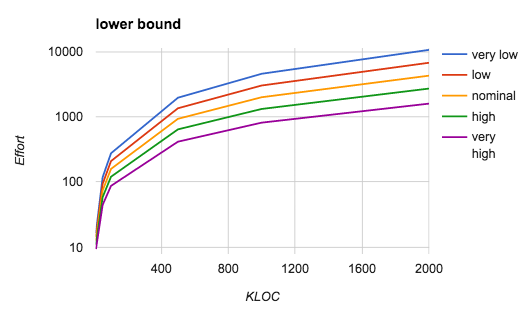
\includegraphics[width=3.5in]{Figs/lower.png}


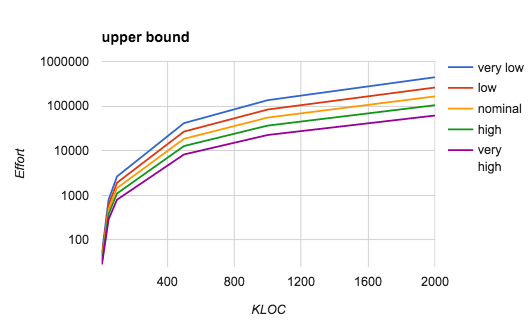
\includegraphics[width=3.5in]{Figs/upper.png} 
\caption{Growth in effort estimates as source code grows. Growth rate determined by \eq{sf3}. 
``Lower bound'' is the most optimistic projection (effort grows slowest as LOC increases)
while ``Upper bound is most pessimistic.
For example, in `upper bound'' for ``very low'', $\mathit{effort} = \mathit{KLOC}^{1.71}$ (where 1.71 is the top-right figure of \eq{sf3}. }\label{fig:lowerupper}
\end{figure}
 


\subsection{RQ4: What is the net effect of errors with KSLOC on estimation
versus error in other attributes?}\label{sect:rq4}


Note that, from \eq{cocII},
the minimum  
effort  is bounded by the  {\em sum} of the minimum scale factors
and the {\em product} of the minimum effort multipliers.
Similar expressions hold for the  maximum effort estimate. Hence,
for a given KLOC, the range of values is given by:
\[
0.057*\mathit{KSLOC}^{0.97}  \le \mathit{effort} \le 115.6*\mathit{KSLOC}^{1.71}\]
(The exponents in the this expression come from \eq{sf3}. The linear terms come
from the product of the min/max effort multipliers from the 
the COCOMO-II text~\cite{boehm00b}).

Dividing the minimum and maximum values results in an  expression showing
how    effort can vary for any given KLOC due to variations in the effort multipliers
and scale factors: 
\begin{equation}\label{eq:ration}
115.6/0.057 *\mathit{KSLOC}^{1.71 - 0.97} = 2028*\mathit{KSLOC}^{0.74}
\end{equation}
Note the very large linear term (2028) coming from the effort multipliers and the
small exponential term (0.74) coming from the scale factors that acts on the KSCOC estimate. The lesson of \eq{ration}
is that errors in KSLOC can have less of an impact on effort predictions than
errors in COCOMO's effort multipliers. Hence, as seen in \tion{rq1}, it is possible
that errors in KSLOC will not be a major cause of estimatione errors.